% chap2.tex (Definitions)

\chapter{Smart Grid and PowerTAC Competition}

In this chapter, I will describe Smart Grid and PowerTAC competition.

\section{Traditional Energy Distribution and Consumption System}
In traditional electricity generation system there are three subsystems \cite{fang2012smart}. In electricity generation subsystem, the generator rotates a turbine in magnetic field which generates electricity. The turbine rotates through the power of kinetic energy of water falling from a water fall or a river with strong current, or from the energy of nuclear powerplan or energy received from burning coal or oil. Traditional energy generation system then transmits the electricity through transmission grid and electricity gets distributed in the distribution grid. This generation system is one way meaning a single power generation source serves several consumption source.



\section{Smart Grid}
In contrast to the traditional electricity generation system, Smart Grid (SG) are two way \cite{fang2012smart}. So, any node in the distribution grid can produce electricity and push it to the distribuiton grid if necessary. The NIST report \cite{fang2012smart} states that the SG would make the electricity generation and supply robust against generator or distribution node failure, use renewable energy widely and efficiently, reduce green house gas emission, reduce oil consumption by encouraging usage of electric vehicles, it will give customers more freedom to choose among energy sources. Smart grids will encourage usage of electric vehicle as these vehicles have the ability to store power in a battery and transmit the power to the distribution grid if there is a necessity. The major challenge with the usage of renewable energy is it is uncertain. This uncertainity causes the ability to predict how much energy the SG can produce in a future time slot hard. Success of SG will need efficient methods to predict energy production \cite{potter2009building}.


\section{Smart Grid and Renewable Energy}
One of the major focus of Smart Grid(SG) will be using renewable energy. There are challenges involved with using this abundant source of energy \cite{richter2012transitioning}. People are already showing strong motivation to use renewable energy as indicated by the statistics that 20\% of total energy is from the renewable sources which is second after coal 24\%. People are using renewable energy due to economic reward and environmental concern. Major challenge with Renewable energy is amount of the energy produced is greatly varying. Since the energy produced is volatile there must be a storage mechanism that balances out the surplus energy. The usage of rechargeable electric vehicles might serve the purpose of storage. Accurate prediction of the renewable energy might enable the electric car users to absorb surplus energy and push it back to the grid in peak hours if necessary. 




\section{Importance of accurate load forecasting}.
Accurate load forecasting is important to ensure efficient fuel usage, reduce wastage of energy and planning proper operation of power generators \cite{liu2006accurate}.


\section{PowerTAC System}
PowerTAC competition which is the abbreviation of Power Trading Agent Competition, is a low risk system that simulates a smart grid based energy system. The powerTAC simulation has several compoents such as wholse sale market, broker, customers and weather service. The system is trained on customers behaviour of several past years and uses real weather data from the past. The following sections give brief explanation of each subsystem.

\subsection{Broker}
Brokers represent the entities that buys energy from the wholesale market and sells to the customers. Contestants implement their own brokers. Each broker's objective is to maximize its profit. A successful broker has to buy and sell energy in a profitable way. Presence of several brokers in the system makes the environment competitive and every broker has to come up with a way to attract the customers. 

\subsection{Wholesale Market}
Wholesale market is the bidding place for buying energy. Brokers submit their bids for a future timeslot in the wholesale market. If the bid was successful, the broker receives its desired amount by paying certain amount of money. 

\subsection{Customers}
A customer represents an entity that buys energy from the brokers. Customers subscribe to the tariffs that the brokers publish. The customers chooses the most suited and affordable tariff for them by evaluating the existing tariffs in the market. They have to pay certain amount of money to the brokers based on their tariff plans and energy usage.

\subsection{Balancing Market}
Balancing market represents the market from where the broker can buy energy in case of emergency. For example, if a broker has bought less amount of energy for a given timeslot and it finds it needs more energy then it can buy the necessary amount of energy from the balancing market. Usually, the balancing market transactions are costly for brokers than the wholesale market.

\subsection{Weather Service}
The weather service broadcasts weather forecast to the brokers. Many customer's energy usage varies based on the weather. The PowerTAC system uses the real weather data from the past.

Figure \ref{fig:simulation-environment}  shows a block diagram of the components of the powerTAC simulation environment.

\begin{figure}[h!]
  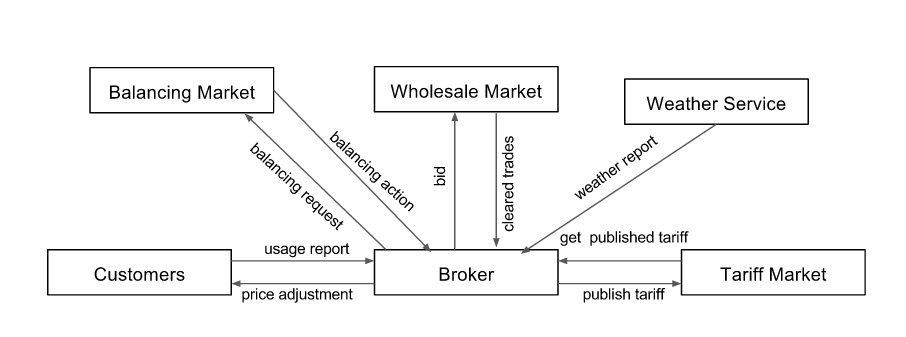
\includegraphics[width=\linewidth]{simulation-environment.png}
  \caption{PowerTAC simulation Environment.}
  \label{fig:simulation-environment}
\end{figure}

%%% Local Variables: 
%%% mode: latex
%%% TeX-master: "thesis"
%%% End: 
